\chapter{Fundamentação Teórica}
Neste capítulo serão mostrados os conceitos matemáticos necessários para a geração desses parâmetros.

%
% ARITMÉTICA MODULAR
%
\section{Aritmética Modular}
Na Teoria dos Números \cite{Niven:2014} (ramo da matemática pura que estuda os números inteiros), uma importante ferramenta é a aritmética modular,  a qual estuda as propriedades de conjuntos formados a partir dos restos da divisão de números inteiros por um inteiro $n$, denominado módulo.

Dado qualquer inteiro positivo \(n\) e qualquer inteiro não negativo \(a\), se dividirmos \(a\) por \(n\), obteremos um quociente inteiro \(q\) e um resto inteiro \(r\), que obedecem ao seguinte relacionamento:
\begin{equation}
  a=qn+r \qquad 0 \leq r<n;\ q=\lfloor a/n \rfloor
\end{equation}

onde $\lfloor x \rfloor$ é o maior inteiro menor ou igual a \(x\).

Uma congruência é  uma relação entre dois números inteiros que, quando divididos por um mesmo número (chamado de módulo da congruência), deixam o mesmo resto.  Em termos formais, dois números inteiros \(a\) e \(b\) são congruentes módulo \(n\) se n divide a diferença \(a - b\).  Esta relação pode ser expressa por:

\begin{equation}
  a \equiv b \pmod n \label{eq:1}
\end{equation}

Para um inteiro positivo \(n\) e \(a\), \(b\), \(c\) inteiros quaisquer, a congruência tem as seguintes propriedades \cite{Stallings:2011}:
\begin{enumerate}
  \item $a \equiv b \pmod n$ se $n|(a-b)$.
  \item $a \equiv b \pmod n$ implica $b \equiv a \pmod n$.
  \item $a \equiv b \pmod n$ e $b \equiv c \pmod n$ implica $a \equiv c \pmod n$.
\end{enumerate}

Por definição, o operador $\pmod n$ mapeia todos os inteiros para o conjunto de inteiros $\{0, 1, ..., (n-1)\}$. Daí pode-se realizar operações aritméticas dentro dos limites desse conjunto, técnica conhecida como aritmética modular. A aritmética modular exibe as seguintes propriedades \cite{Stallings:2011}:
\begin{enumerate}
  \item $[a \pmod n + b \pmod n] \pmod n = (a + b) \pmod n$
  \item $[a \pmod n - b \pmod n] \pmod n = (a - b) \pmod n$
  \item $[a \pmod n \times b \pmod n] \pmod n = (a \times b) \pmod n$
\end{enumerate}

Em relação a divisão, ela não está definida em todos os casos. Se \(d\) é um inteiro que divide \(a\) e \(b\), então vale a relação apresentada na Equação \ref{eq:5}, onde \((n, d)\) é o maior divisor comum entre \(n\) e \(d\).

\begin{equation}
  \frac{a}{d} \equiv \frac{b}{d}\left(\mbox{mod}\ \frac{n}{(n,d)}\right) \label{eq:5}
\end{equation}

O inverso multiplicativo de a modulo \(n\), isto é, um inteiro \(b\) tal que \(a \times b = 1 \pmod  n\), existe apenas quando \((a, n) = 1\) (isto é, $a$ e $n$ são coprimos). O valor de \(b\) pode ser obtido através do Algoritmo de Euclides Estendido \cite{Halim:2013}.
\par A exponenciação modular calcula o resto de um número inteiro \(b\) quando elevado à um número inteiro \(k\) e é dividido por um inteiro positivo \(m\). Escolhidos a base \(b\), o expoente \(k\) e o módulo \(m\), uma exponenciação modular \(c\) é dada pela Equação \ref{eq:6}.

\begin{equation}
  c \equiv b^{k}\pmod m \label{eq:6}
\end{equation}

%
% ESTRUTURAS ALGÉBRICAS
%
\section{Estruturas Algébricas}

Antes de iniciar os estudos em aritmética de curvas elípticas, é importante
fixar alguns conceitos de álgebra. De acordo com \cite{Hefez:2008}(p. 12),

\begin{citacao}
Estruturas algébricas são modelos abstratos para tratar em bloco várias situações matemáticas concretas em que em determinados conjuntos são definidas operações com propriedades semelhantes.
\end{citacao}

Nesse trabalho serão abordadas as estruturas algébricas grupo
e corpos finitos.

%
% GRUPOS
%

\subsection{Grupos}

Um \textbf{grupo \((G,*)\)} é composto por um conjunto \(G\) e uma operação binária \(*\) sobre os elementos desse conjunto tal que os axiomas abaixo sejam satisfeitos\cite{Gilbert:2004}

\begin{enumerate}
\item O conjunto \(G\) é \textbf{fechado} para a operação \(*\)

$a * b \in G$ para todo $a,b \in G$.

\item A operação $*$ é \textbf{associativa}

$(a * b) * c = a * (b * c)$ para todo $a,b,c \in G$.

\item Existe um \textbf{elemento identidade} $e \in G$ tal que para todo elemento $a \in G, a * e = a$.
\item Existe um \textbf{elemento inverso} $a'$ para todo elemento $a \in G$ tal que $a' * a = e$ (elemento identidade).
\end{enumerate}

Se a operação é \textbf{comutativa}, ou seja, se $a * b = b * a$ para todo $a, b \in G$, então o grupo é denominado \textbf{abeliano}(ou \textbf{comutativo}) em homenagem ao matemático Niels Abel. \cite{Gilbert:2004}

Exemplos de grupos abelianos são $(Z, +)$, $(R, +)$, ambos com identidade 0 e com infinitos elementos. "O numero de elementos de um grupo é a sua \textbf{ordem}"\cite{Coutinho:2014}(pg. 134). Para este trabalho, os grupos de maior interesse são aqueles que possuem ordem finita.

\subsection{Subgrupos}
Seja $(G,*)$ um grupo, e $H$ um subconjunto não vazio de $G$. Se $(H,*)$ satisfaz todos os axiomas de grupo, então diz-se que $(H, *)$ é um subgrupo de $(G, *)$\cite{Coutinho:2014}, ou seja

\begin{enumerate}
\item Para todo $a, b \in H$, $a * b \in H$.
\item O elemento neutro de $G$ está em $H$ e também é seu elemento neutro(a demonstração não será feita nesse trabalho).
\item Existe um inverso $a'$ para todo $a \in H$.
\end{enumerate}

Todo grupo possui pelo menos dois subgrupos, como pode ser visto na citação abaixo.\cite{Domingues:2003}(pg. 154)


\begin{citacao}
''Se $e$ indica o elemento neutro de $G$, então obviamente ${e}$ é um subgrupo de $G$. É imediato, também, que o próprio $G$ é um subgrupo de si mesmo. Esses dois subgrupos, ou seja, ${e}$ e $G$, são chamados de \textbf{subgrupos triviais} de $G$''.
\end{citacao}

%
% CORPOS FINITOS
%
\subsection{Corpos Finitos}

%
% CRIPTOGRAFIA
%
\section{Criptografia} \label{sec:criptografia}
``Criptografia é a ciência que trata de cifrar a escrita, de modo a torná-la ininteligível para os que não tenham os métodos convencionados para ter acesso a ela. Em Tecnologia da Informação, esta definição é ampliada a fim de englobar não só a escrita, mas qualquer tipo de documento ou dados que devam ser tratados secretamente. Um Sistema de Criptografia define um sistema em que um texto (ou documento, ou qualquer tipo de dado) é transformado através da criptografia em um texto cifrado (ciphertext) ou o texto cifrado é transformado de volta à informação original, através de algoritmos. A primeira ação é denominada cifragem ou criptografar, e a segunda é chamada de decifração ou decriptação.'' \cite{Portnoi:2005}

%
% CRIPTOGRAFIA SIMÉTRICA
%
\subsection{Criptografia simétrica}

%
% CRIPTOGRAFIA ASSIMÉTRICA
%
\subsection{Criptografia assimétrica}

%
% CURVAS ELÍPTICAS
%
\section{Curvas Elípticas}
Curvas elípticas não são elipses. Elas têm esse porque são descritas por equações cúbicas, semelhantes às usadas para calcular a circunferência de uma elipse. Em geral, as equações cúbicas para curvas elípticas têm a forma
\begin{equation}
y^2 + axy + by = x^3 + cx^2 + dx + e \label{eq:11}
\end{equation}
onde \(a, b, c, d\) e \(e\) são números reais e \(x\) e \(y\) assumem valores nos números reais. Equações deste tipo são chamadas de \textit{equações de Weiestrass}. Para a nossa finalidade, é suficiente limitarmos na forma normal da equação de Weiestrass
\begin{equation}
y^2 = x^3 + ax + b \label{eq:12}
\end{equation}

Essas equações são consideradas cúbicas, ou de grau 3, pois o expoente mais alto que elas contém é um 3. Também incluído na definição de uma curva elíptica está um único elemento indicado por \(O\) e chamado de \textit{ponto no infinito} ou \textit{ponto zero}.

A Figura \ref{fig:curvas} apresenta alguns exemplos de curvas elípticas usando a forma normal da equação de Weierestrass.

\begin{figure}[h]
\centering
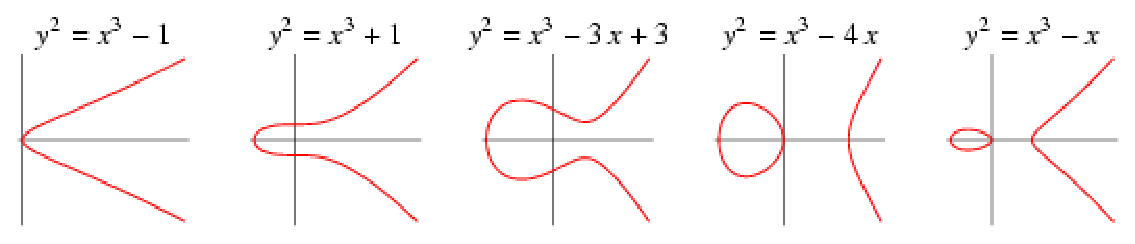
\includegraphics[scale=0.5, bb=0 0 529 101]{figuras/curvas.eps}
\caption{Exemplos de curvas elípticas}
\label{fig:curvas}
\end{figure}


Podemos mostrar que um grupo pode ser definido com base no conjunto E(\(a, b\)) para valores específicos de \(a\) e \(b\) na Equação \ref{eq:12}, desde que a condição a seguir seja atendida:
\begin{equation}
4a^3 + 27b^2 \neq 0 \label{eq:13}
\end{equation}

Uma importante característica da curvas elípticas é que existe uma forma natural de ``somar'' dois pontos produzindo um terceiro ponto. Para tanto, deve-se satisfazer a Equação \ref{eq:13}. No entanto, esta ``soma'' se refere à operação que combina dois pontos de maneira análoga da soma algébrica em alguns aspectos (é comutativa, associativa e existe um elemento identidade), mas bem diferente em outras formas.

Em termos geométricos, as regras para a adição podem ser indicadas da seguinte maneira: se três pontos em uma curva elíptica se encontram em uma linha reta, sua soma é \(O\). Por essa definição, podemos definir as regras da adição sobre uma curva elíptica:

\begin{figure}[h]
\centering
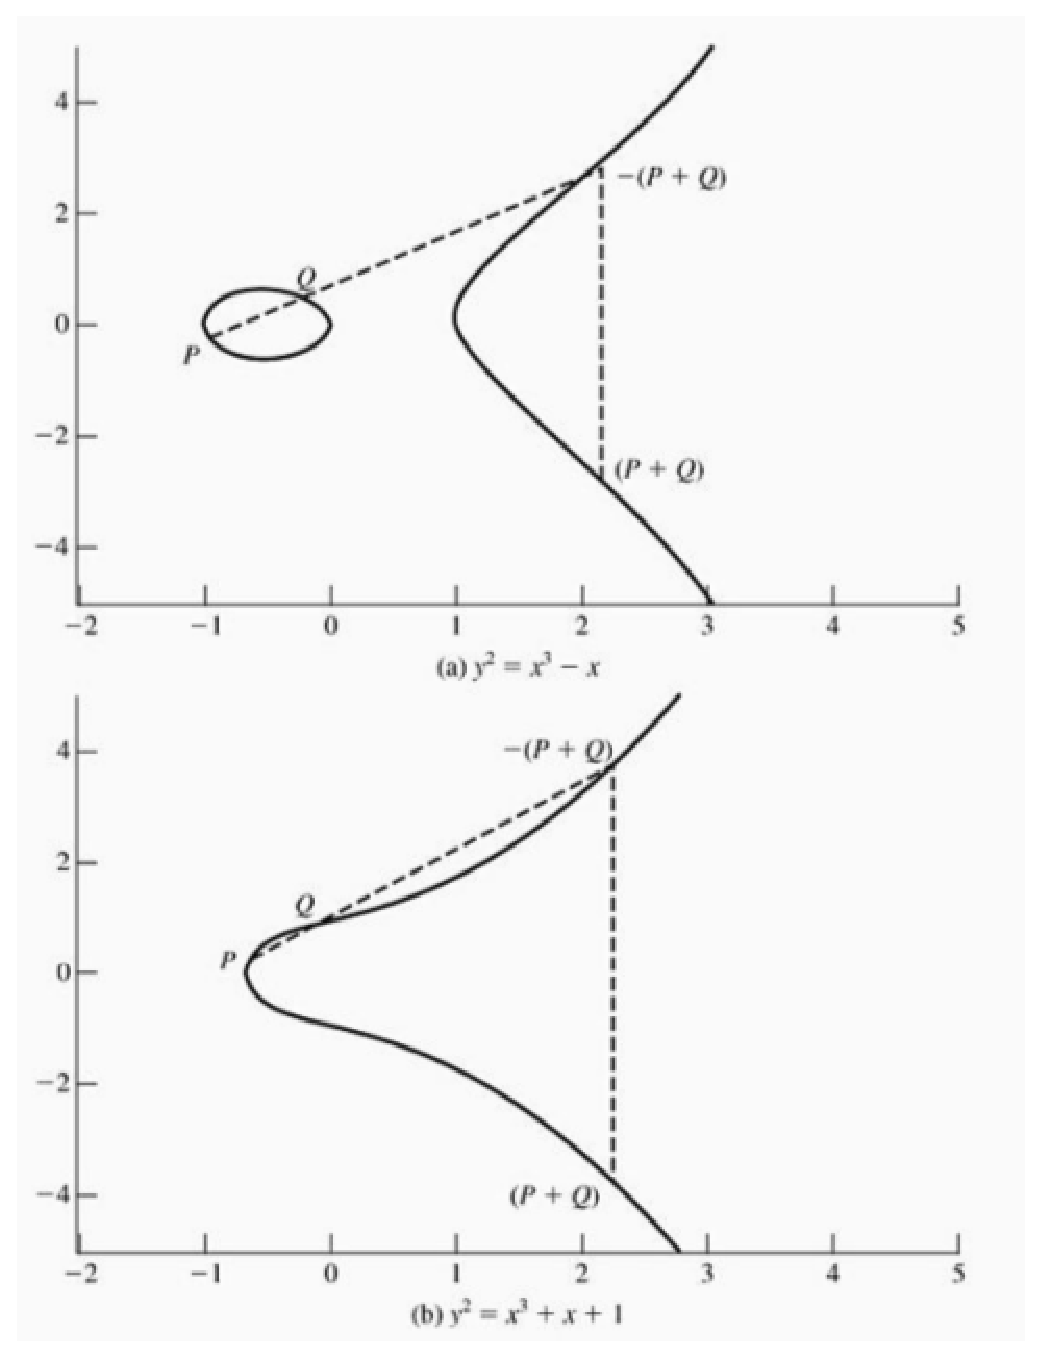
\includegraphics[scale=0.5, bb=0 0 484 636]{figuras/pontos_curva.eps}
\caption{Exemplos de soma de pontos em curvas elípticas}
\label{fig:pontos}
\end{figure}

\begin{enumerate}
	\item $O$ funciona como a identidade aditiva. Assim, $O = -O$; para qualquer ponto $P$ na curva elíptica, $P + O = P$. A seguir, consideramos $P \neq O$ e $Q \neq O$.
	\item O negativo de um ponto \(P\) é o ponto com a mesma coordenada \(x\), sem o negativo da coordenada \(y\); ou seja, se $P=(x,y)$, então $-P=(x,-y)$. Observe que esses dois pontos podem ser juntados por uma linha vertical. Observe que $P+(-P)=P-P=O$.
	\item Para somar dois pontos \(P\) e \(Q\) com coordenadas \(x\) diferentes, desenhe uma linha reta entre eles e encontre o terceiro ponto de interseção \(R\). Pode-se ver facilmente que existe um único ponto \(R\) que é o ponto de interseção (a menos que a linha seja tangente à curva em \(P\) ou \(Q\), quanto consideramos $R=P$ ou $R=Q$, respectivamente). Para formar uma estrutura de grupo, precisamos definir a adição sobre três pontos da seguinte forma: $P+Q=-R$. Ou seja, definimos $P+Q$ como sendo a imagem-espelho (com relação ao eixo \(x\)) do terceiro ponto da interseção. A figura \ref{fig:pontos}
	\item A interpretação geométrica do item anterior também se aplica a dois pontos, \(P\) e \(-P\), com a mesma coordenada \(x\). Os pontos são reunidos por uma linha vertical, que também pode ser vista como a interseção da curva no ponto infinito. Portanto, temos $P+(-P)=O$, coerente com o item (2).
	\item Para dobrar um ponto \(Q\), desenhe uma linha tangente e encontre o outro ponto da interseção \(S\). Então, $Q+Q=2Q=-S$.
\end{enumerate}

Com a lista de regras apresentada, pode-se se mostrar que o conjunto E(\(a, b\)) é um grupo abeliano. \cite{Stallings:2011}

%
% CRIPTOGRAFIA DE CURVAS ELÍPTICAS
%
\section{Criptografia de curvas elípticas}
